% no answer key
% \documentclass[letterpaper]{exam}

% answer key
\documentclass[letterpaper, landscape]{exam}
\usepackage{2in1, lscape} 
\printanswers

\usepackage{units} 
\usepackage{xfrac} 
\usepackage[fleqn]{amsmath}
\usepackage{float}
\usepackage{mdwlist}
\usepackage{booktabs}
\usepackage{cancel}
\usepackage{polynom}
\usepackage{caption}
\usepackage{fullpage}
\usepackage{comment}
\usepackage{enumerate}
\usepackage{graphicx}

\usepackage{mathtools} 

\newcommand{\dg}{\ensuremath{^\circ}} 
\newcommand{\sgn}{\operatorname{sgn}}

\everymath{\displaystyle}
\title{Calculus I \\ Homework Five \\ Section 2.5}
\author{}
\date{\today}

\begin{document}

  \maketitle

  \section{Homework}
    \begin{itemize*}
      \item read Section 2.5
      \item exercises: 1, 3-6, 9, 16-17, 21-22, 25, 35, 37, 40-41, 45, 61, 63, 65
    \end{itemize*}

  \ifprintanswers

  \section{Solutions}

    \begin{description}

      \item[1] $\lim_{x \to 4} f(x) = f(4)$

      \item[3] 
        \begin{itemize}
          \item $-4$ because $f(-4)$ is not defined

          \item $-2$, $2$ and $4$ because the limit is not defined or is different
            depending on the direction

          \item $-2$ is continuous from the left and $2$ and $4$ are continuous from the
            right.

        \end{itemize}

      \item[4] $f$ is continuous on $[-4, -2)$, $(-2, 2)$, $[2, 4)$, $(4, 6)$ 
          and $(6, 8)$.

      \item[5] graph

      \item[6] graph

      \item[9] Since $f$ is continuous and $f(3) = 5$, $\lim_{x \to 3} f(x) = 5$.

        \begin{align*}
          \lim_{x \to 3} \left[ 2 f(x) - g(x) \right] & = 4 \\
          10 - \lim_{x \to 3} g(x)                    & = 4 \\
          \lim_{x \to 3} g(x)                         & = 6 \\
        \end{align*}

      \item[16] 
        \[
          \lim_{x \to -1^-} f(x) \neq \lim_{x \to -1^+} f(x) \neq f(x)
        \]

      \item[17] 
        \[
          \lim_{x \to 0^-} f(x) \neq \lim_{x \to 0^+} f(x) 
        \]

      \item[21] This is a rational function, so by Theorem 5 it is continuous everywhere
        in its domain.

      \item[22] 
        
        $\sqrt[3]{x}$ is a root function so it is continuous everywhere in its
        domain by Theorem 7.

        $1 + x^3$ is a polynomial so it is continuous everywhere by Theorem 5.

        $G(x)$ is a product of two continuous functions, so it is continuous
        everywhere in its domain by Theorem 4.

      \item[25] 
        
        $e^{-5t}$ is an exponential function so it is continuous everywhere 
        by Theorem 7.

        $\cos 2 \pi t$ is a trigonometric function so it is continuous
        everywhere by Theorem 7.

        $L(x)$ is a product of two continuous functions, so it is continuous
        everywhere in its domain by Theorem 4.

      \item[35] $x^2$ and $\sqrt{x}$ are continuous everywhere in their domains
        by Theorem 7.

        The only possible discontinuity would be at $x = 1$.
        \begin{align*}
          \lim_{x \to 1^-} f(x) & = \lim_{x \to 1^-} x^2 = 1 \\
          \lim_{x \to 1^+} f(x) & = \lim_{x \to 1^+} \sqrt{x} = 1 \\
          f(1)                  & = \sqrt{1} = 1 \\
        \end{align*}

        because:
        \[
          \lim_{x \to 1^-} f(x) = \lim_{x \to 1^+} f(x) = f(1) 
        \]

        $f$ is continuous at $x = 1$ and $f$ is continuous on $(-\infty, \infty)$

      \item[37] The only possible discontinuities are at $x = 0$ and $x = 2$.

        \begin{figure}[H]
          \centering
          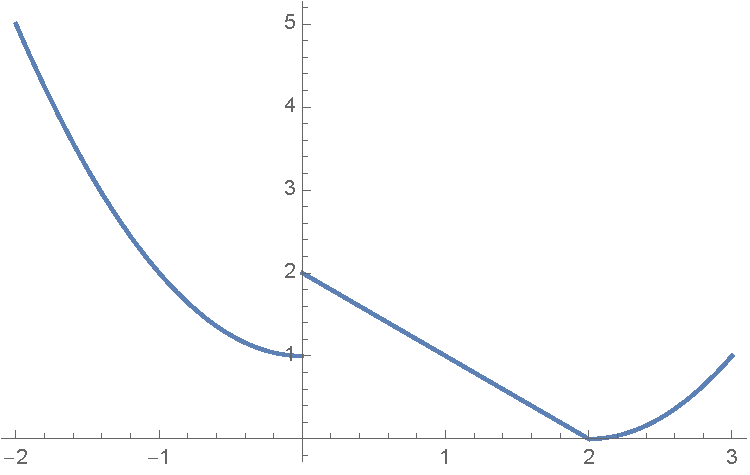
\includegraphics[scale = 0.5]{ex37.pdf}
          \caption{Exercise 37}
          \label{fig:ex37}
        \end{figure}

        \begin{align*}
          \lim_{x \to 0^-} f(x) & = 1 \\
          \lim_{x \to 0^+} f(x) & = 2 \\
          \\
          \lim_{x \to 2^-} f(x) & = 0 \\
          \lim_{x \to 2^+} f(x) & = 0 \\
          f(2)                  & = 0 \\
        \end{align*}

        $f$ is discontinuous at $x = 0$ and continuous everywhere else.

        See Figure \ref{fig:ex37}.

      \item[40]
        The only possible discontinuity is at the surface of the earth where $r = R$. For this point:
        \begin{align*}
          \lim_{r \to R^-} F(r) & = \frac{GMR}{R^3} = \frac{GM}{R^2} \\
          \lim_{r \to R^+} F(r) & = \frac{GM}{R^2} \\
          F(R)                  & = \frac{GM}{R^2} \\
        \end{align*}

        Since
        \[
          \lim_{r \to R^-} F(r) = \lim_{r \to R^+} F(r) = F(R)
        \]

        $F$ is continuous everywhere on its domain. For this function, non-positive
        numbers don't make sense, so the domain is $(0, \infty)$.

      \item[41]
        We need to find a value of $c$ where the two pieces of the function will have the
        same value for $x = 2$:

        \begin{align*}
          2^2 c + 2 \cdot 2 & = 2^3 - 2c \\
          c                 & = \frac{2}{3} \\
        \end{align*}

        This value makes the function:
        \[
          f(x) = 
            \begin{cases}
              \frac{2}{3} x^2 + 2x & \text{if } x < 2 \\
              x^3 - \frac{2}{3} x  & \text{if } x \geq 2 \\
            \end{cases}
        \]

        $\lim_{x \to 2} f(x) = f(2) = \frac{20}{3}$

      % \item[43]
      %   \begin{enumerate}[(a)]
      %     \item 
      %       \begin{align*}
      %         \frac{x^4 - 1}{x - 1} & = (x + 1)(x^2 + 1) \\
      %         \lim_{x \to 1} f(x)   & = 4 \\
      %       \end{align*}
      %   \end{enumerate}

      %   \[
      %     g(x) = 
      %       \begin{cases}
      %         f(x) & \text{if } x \neq 1 \\
      %         4    & \text{if } x = 1 \\
      %       \end{cases}
      %   \]

      \item[45]
        \begin{align*}
          f(0) &= 0 \\
          f(100) &= 10,000 + 10 \sin 100 > 1000
        \end{align*}

        By the Intermediate Value Theorem, there has to be some value of $x$ between
        $0$ and $100$ where $f(x) = 1000$.

      \item[61]
        Let $f(x)$ be the difference between the number and its cube:
        \[
          f(x) = x - x^3  \\
        \]

        Since:
        \begin{align*}
          f(-2) &= 6 \\
          f(-1) &= 0 \\
        \end{align*}

        By the Intermediate Value Theorem, there is some value of $x$ between $x = -1$ and
        $x = -2$ where $f(x) = 1$

        According to my computer, a value of $x \approx -1.32472$ is about right.

      \item[63]
        By Theorem 9, $f(x)$ is continuous everywhere except possibly $x = 0$, since it is
        a composition of two functions which are continuous everywhere except $x = 0$.

        We can use the Squeeze Theorem to determine if $f(x)$ is also continuous at
        $x = 0$.

        \[
          -x^4 \leq x^4 \sin \left( \frac{1}{x} \right) \leq x^4
        \]

        \begin{align*}
          \lim_{x \to 0} -x^4 = \lim_{x \to 0} x^4 = 0
        \end{align*}

        By the Squeeze Theorem: $\lim_{x \to 0} x^4 \sin \left( \frac{1}{x} \right) = 0$

        Since $\lim_{x \to 0} f(x) = f(0)$, $f$ is continuous at $x = 0$.

      \newpage

      \item[65]
        Picture two monks making the trip on the same day. Both monks start at 7:00 AM
        with one monk starting from the top of the mountain and the other monk starting
        from the bottom of the mountain. The monks will pass each other on the path some
        time during the day, regardless of how fast they walk.

        In math terms, you can define two functions which give monk distance traveled as a
        function of time. The first function ($f_1$), for day one, starts at distance 0 at
        $t = 0$ and ends at distance $D$ (the total distance) at $t = 12$. The second
        function ($f_2$), for day two, starts at distance $D$ at $t = 0$ and ends at
        distance 0 at $t = 12$.

        Both functions are continuous since the monk doesn't have access to a Star Trek
        transporter.

        Define a new function which is the difference between the two original functions:
        \[
          d(t) = f_2(t) - f_1(t)
        \]

        $d(t)$ is continuous since it is the difference of two continuous functions.
        
        Since $d(0)$ = D and $d(12) = -D$, by the Intermediate Value Theorem there must
        be some time between 0 and 12 where $d(t) = 0$ and the monk is at the same place
        at the same time on the second day as he was on the first day.

    \end{description}

  \else
    \vspace{10 cm}
    \begin{quote}
      \begin{em}
        In long intervals I have expressed an opinion on public issues whenever they
        appeared to me so bad and unfortunate that silence would have made me feel guilty
        of complicity. 
      \end{em}
    \end{quote}
    \hspace{1 cm} --Albert Einstein
  \fi

\end{document}

